\documentclass[12pt]{article}
\usepackage{fullpage,graphicx,psfrag,amsmath,amsfonts,verbatim}
\usepackage[small,bf]{caption}
\usepackage{amsthm}
% \usepackage[hidelinks]{hyperref}
\usepackage{hyperref}
\usepackage{bbm} % for the indicator function to look good
\usepackage{color}
\usepackage{mathtools}
\usepackage{fancyhdr} % for the header
\usepackage{booktabs} % for regression table display (toprule, midrule, bottomrule)
\usepackage{adjustbox} % for regression table display
\usepackage{threeparttable} % to use table notes
\usepackage{natbib} % for bibliography
\input newcommand.tex
\bibliographystyle{apalike}
% \setlength{\parindent}{0pt} % remove the automatic indentation

\title{L'Hôpital's (Selection) Rule:\\{\large {An Empirical Bayes Application to French Hospital Efficiency}}}
\author{Fu Zixuan \\{\small {Supervised by Thierry Magnac}}}
\date{July 4, 2024}

\begin{document}
\maketitle
\thispagestyle{empty}
\begin{abstract}
    \noindent  There has been ongoing interest in comparing public and private hospitals. Inspired by the nascent study of \citet{croiset2024hospitals}, which investigates labor employment efficiency in four types of French hospitals, this article aims to identify the top-performing units in the same aspect. By borrowing strength from the compound decision framework and the non-parametric likelihood estimator \citep{kiefer1956consistency}, it derives the decision rule for selecting meritorious hospitals following the work of \citet{gu2023invidious}. Selection outcomes are later compared across different scenarios. A preliminary conclusion can be drawn from the selection results. Though ranking and selection are both tempting to perform, such decisions need to be made with great caution.\\

    % \noindent\textbf{Keywords:} \\

    \bigskip
\end{abstract}

\newpage
\thispagestyle{empty}
\tableofcontents
\newpage

\setcounter{page}{1}
\section{Introduction}

It is almost human nature to compare, rank, and select.And competition, be it
good or bad, emerges in its wake. As invidious as ranking and selection may be,
they often serve as key drivers of performance improvement. Society itself
continuously constructs league tables, rewarding the meritorious while
questioning or even punishing the unsatisfactory. The objects of interest for
ranking vary widely, from teacher evaluations \citep{chetty2014measuring} and
community mobility indices \citep{chetty2018impacts} to assessments of firm
discrimination \citep{kline2022systemic}.

This article extends such practices to the healthcare sector. Specifically, it
examines labor efficiency across all hospitals in France. Utilizing a
comprehensive database, \textit{The Annual Statistics of Health Establishments
    (SAE)}, I first construct a measure of labor efficiency. Then, using estimates
derived from this data, I compare public and private hospitals by selecting the
top-performing units. I leverage recent developments in the Empirical Bayes
method to facilitate this comparison.

I found that among the top 20\% of best-performing hospitals, there are roughly
six times more private units than public ones, adjusted for the number of
hospitals in each category. The difference becomes even more pronounced when
controlling for the expected number of incorrect selections. The conclusion is
that public hospitals generally exhibit less efficiency than their private
counterparts, aligning with the findings of \cite{croiset2024hospitals}.
However, we now have a more granular perspective on the performance comparison.

The article bridges two fields of interest. The first focuses on productivity
analysis, where the most popular methodologies are Data Envelopment Analysis
\citep{charnes1978measuring} and Stochastic Frontier Analysis
\citep{aigner1977formulation,meeusen1977efficiency}. However, I diverge from
these approaches and adopt the \textit{conditional input demand function}
specification detailed in \cite{croiset2024hospitals}.\footnote{I refer the
    reader to \citet{croiset2024hospitals} for detailed reasons behind this
    choice.} Simply put, we estimate a linear function that determines the
necessary labor input to produce a given list of eight hospital outputs. My
focus is specifically on the employment level of nurses, as unlike medical
doctors, this category does not suffer from a shortage of labor supply.

The second area of interest is Empirical Bayes Methods. I draw upon a series of
works by Jiaying Gu and Roger Koenker, primarily the following two papers:
\citet{gu2017empirical} discusses the usefulness of estimating a prior
distribution in baseball batting average prediction, while
\citet{gu2023invidious} formally defines the selection problem as a compound
decision, where the estimated prior can be helpful. Additionally,
\citet{kiefer1956consistency} demonstrates that non-parametric maximum
likelihood estimation of the prior is feasible and consistent. The computation
of NPMLE has been significantly improved by \citet{koenker2014convex},
leveraging recent developments in convex optimization
\citep{andersen2010mosek}. For my analysis, I will use the \verb+REBayes+
package \citep{koenker2017rebayes}, which is based on the \verb+MOSEK+ software
developed by \citet{andersen2010mosek}.

In \cite{croiset2024hospitals}, the authors argue that public hospitals are
less efficient than their private counterparts, in the sense that a public
hospital would require a smaller workforce if it adopted the input demand
function used by private hospitals—a key finding from their counterfactual
analysis.

Having approximately replicated these results with an extended panel length,
this paper differentiates itself by employing classical panel data methods for
estimating the input demand function, specifically standard fixed-effect
estimation and GMM. While incorporating individual fixed effects into the
specification is straightforward, the estimation process is not without
challenge. For instance, as \citet{croiset2024hospitals} have noted,
within-hospital variation is much smaller than between-group variation, which
may be insufficient for obtaining reliable estimates. To address this issue, I
extended the panel length, aiming to enhance the robustness of the estimates.
Furthermore, the strict exogeneity assumption required by standard within-group
estimation is debatable. A practical solution to relax this assumption is to
use the first difference GMM estimator, as proposed by
\citet{arellano1991some}. Another challenge arises from the high persistency of
the regressors, which can lead to weak instruments. In response, I adapted and
implemented the system GMM approach, as modified by \citet{arellano1995another}
and \citet{blundell1998initial}, using the resulting estimates for subsequent
analyses.

The advantage of the panel data estimator lies in its ability to capture the
underlying heterogeneity, which opens the door to individual comparisons. The
fixed effect estimates are generally noisy, rendering the ensuing
decision-maker hand-wavy. The EB methods are proposed in an attempt to rectify
the situation by empirically estimating the prior distribution of the fixed
effects.

For example, in \cite{gu2023invidious}, we are given the task of selecting the
top 20\% of fixed effects, denoted by $\theta_i$. If $\theta_i$ follows a
distribution $G$, this implies selecting those $\theta_i$ that exceed
$G^{-1}(0.8)$. The decision rule for an individual $i$ is represented by an
indicator function $\delta_i$, which determines whether $i$ belongs to the
selection set. This task aligns with the compound decision framework pioneered
by \cite{herbert1956empirical}, especially when defining the loss function of
the selection problem in a way that incorporates the outcomes of all individual
decisions $\delta_i$:
\begin{equation*}
    \delta^* = \argmin_{\delta} \E_G\E_{\theta|\hat{\theta}}\left(L_n\right).
\end{equation*}
Since the true value of $\theta$ is unknown, we aim to minimize the expected compound loss $L_n$ over the distribution of $\theta$ given the observed $\hat{\theta}$.

In addition to the capacity constraint of selecting the top 20\%,
\citet{gu2023invidious} further mitigates the number of false positive in the
selection process. The false discovery rate (FDR) constraint is imposed to
ensure that the expected number of incorrectly selected units remains below a
specified threshold. The FDR is quantified as the proportion of false positives
among all selected units, formally defined by the condition
$\Pr(h_i=0|\delta_i=1) \leq \gamma$.

Being interested in the top-performing French hospitals, I define my selection
problem as \textit{Left tail selection} because the goal is to choose the
bottom 20\% of the hospital fixed effect $\theta_i$. A smaller $\theta_i$
indicates that less labor input is required to produce the same amount of
output, compared to hospitals with a higher $\theta_i$.

It is worth mentioning that classical empirical Bayes method assumes a
parametric form of the prior distribution $G$ which is computationally more
attractive. Yet thanks to fast convex optimization algorithms, the
non-parametric maximum likelihood estimation is now both feasible and
efficient. Nevertheless, we are completely free from imposing any parametric
assumption. In fact, there are two \textit{layers} of distribution. The lower
hierarchy is the prior $G$ with $\theta\sim G$ while the higher hierarchy is
$\hat{\theta}|\theta \sim P_{\theta}$. It is when $P_{\theta}$ belongs to the
exponential family that the \citet{lindsay1995mixture} results hold. Usually in
application, we need to impose assumptions or perform some transformation such
that $P_{\theta}$ is normal. This kind of procedure is often questionable.
Often times, researchers resort to asymptotics to justify the normality
assumption, which may not be valid in small samples.

It is worth mentioning that the classical empirical Bayes method assumes a
parametric form for the prior distribution $G$, which is computationally
attractive. However, thanks to advancements in fast convex optimization
algorithms, non-parametric maximum likelihood estimation
\citep{kiefer1956consistency} has become both feasible and efficient
\citep{koenker2014convex,andersen2010mosek}. Nonetheless, we are not entirely
free from imposing any parametric assumptions. In fact, there are two layers of
distribution: the lower hierarchy where $\theta \sim G$, and the higher
hierarchy where $\hat{\theta} | \theta \sim P_{\theta}$.
\citet{lindsay1995mixture} has shown that a solution $\hat{G}$ exists and is a
discrete probability measure, with no more than n mass points in the interval
$[\min yi , \max yi ]$. It is when $P_{\theta}$ belongs to the exponential
family that the \citet{lindsay1995mixture} results hold. Typically in
applications, it is necessary to impose assumptions or perform transformations
to make $P_{\theta}$ normal. This procedure is often questionable. Researchers
frequently rely on asymptotic properties to justify the normality assumption,
which may not be valid in small samples.

The remainder of the paper is organized as follows: \textbf{Section 2} briefly
describes the data and outlines the reduced form estimation of the input demand
function, where the number of nurses serves as the dependent variable, with
nine output measures acting as regressors. It then applies classical panel data
estimators to the same specification, examining and later relaxing the
assumptions of strict exogeneity. In \textbf{Section 3}, I introduce the
compound decision framework and describe the methodology for non-parametrically
estimating $G$. \textbf{Section 4} specifically defines the selection problem
following the framework proposed by \cite{gu2023invidious}, and includes a
comparison of different selection outcomes. Preliminary conclusions about the
comparative performance of public versus private hospitals are drawn.
\textbf{Section 5} discusses potential issues and concludes the paper.

\section{Data and Estimation}
\subsection{Data}

The data utilized in this study is from The Annual Statistics of Health
Establishments (SAE), a comprehensive and mandatory administrative survey that
serves as the primary source of data on all health establishments in France
\footnote{\href{https://data.drees.solidarites-sante.gouv.fr/explore/dataset/708_bases-statistiques-sae/information/}{La
        Statistique annuelle des établissements (SAE)}}. Our analysis primarily focuses
on healthcare outputs (across ten different measures) and labor inputs
(specifically registered and assistant nurses). The panel data spans nine
years, from 2013 to 2022, excluding 2020 due to disruptions caused by the
pandemic. The SAE data categorizes establishments into three types based on
their legal status:

\begin{enumerate}
    \item Public hospitals,
    \item Private for-profit hospitals,
    \item Private non-profit hospitals.
\end{enumerate}

In alignment with the categorization used by \citet{croiset2024hospitals}, this
study also distinguishes public teaching hospitals as a separate category,
given their unique role within the French healthcare system.

\begin{table}[h!]\fontsize{10pt}{12pt}\selectfont
    \begin{adjustbox}{width=\textwidth,center}
        \centering
        % latex table generated in R 4.2.1 by xtable 1.8-4 package
% Tue Jun 18 19:02:10 2024
\begin{tabular}{rrrrrrr}
  \toprule
 & AN & Teaching & Normal Public & Private For Profit & Private Non Profit & Total \\ 
  \midrule
1 & 2013.00 & 198 & 1312 & 1305 & 1382 & 4197.00 \\ 
  2 & 2014.00 & 201 & 1274 & 1293 & 1349 & 4117.00 \\ 
  3 & 2015.00 & 211 & 1275 & 1297 & 1349 & 4132.00 \\ 
  4 & 2016.00 & 212 & 1266 & 1297 & 1313 & 4088.00 \\ 
  5 & 2017.00 & 211 & 1249 & 1297 & 1306 & 4063.00 \\ 
  6 & 2018.00 & 214 & 1247 & 1296 & 1288 & 4045.00 \\ 
  7 & 2019.00 & 214 & 1236 & 1287 & 1281 & 4018.00 \\ 
  8 & 2021.00 & 219 & 1222 & 1293 & 1264 & 3998.00 \\ 
  9 & 2022.00 & 220 & 1220 & 1296 & 1259 & 3995.00 \\ 
   \bottomrule
\end{tabular}

    \end{adjustbox}
    \caption{Number of hospitals in each category, 2013-2022}
    \label{tab:hospital_count}
\end{table}

As illustrated in Table \ref{tab:hospital_count}, the distribution of
hospitals—categorized as normal public, private for-profit, and private
non-profit—is relatively equal and remains stable over the years. It is
important to highlight the unique role of teaching hospitals. Unlike other
types of hospitals, teaching hospitals allocate significant resources to doctor
training and research activities. This additional commitment to educational and
research missions generally results in larger institutions. This aspect becomes
evident when examining the output shares of hospitals. Despite their limited
number, teaching hospitals contribute a disproportionately large share of
overall healthcare output, a disparity that becomes more pronounced when
adjusted for the number of facilities, as detailed in Table \ref{tab:output}.

Furthermore, the analysis reveals distinct differences in the mix of service
provided by each type of hospital. Emergency care is mostly taken care of by
public hospitals and private hospitals are strong in medical sessions.

\begin{table}\fontsize{10pt}{12pt}\selectfont
    \begin{adjustbox}{width=\textwidth,center}
        \centering
        \begin{threeparttable}[b]

            % latex table generated in R 4.2.1 by xtable 1.8-4 package
% Sun Jun 23 16:16:45 2024
\begin{tabular}{llllll}
  \toprule
Output & Teaching & Normal Public & Private For Profit & Private Non Profit & Total \\ 
  \midrule
STAC inpatient & 25.17\% & 43.09\% & 23.64\% & 8.1\% & 100\% \\ 
  STAC oupatient & 18.4\% & 19.46\% & 52.95\% & 9.18\% & 100\% \\ 
  Sessions & 14.49\% & 21.96\% & 34.4\% & 29.16\% & 100\% \\ 
  Outpatient Consultations & 36.8\% & 52.45\% & 0.23\% & 10.52\% & 100\% \\ 
  Emergency & 21.4\% & 60.06\% & 13.37\% & 5.17\% & 100\% \\ 
  Follow-up care and Long-term care & 7.6\% & 19.47\% & 37.95\% & 34.98\% & 100\% \\ 
  Home hospitalization & 13\% & 17.38\% & 12.4\% & 57.22\% & 100\% \\ 
  Psychiatry stays & 6.53\% & 62.26\% & 12.93\% & 18.28\% & 100\% \\ 
   \bottomrule
\end{tabular}

            \caption{Hospital share of output, 2013-2022}
            \label{tab:nonadjusted}
        \end{threeparttable}
    \end{adjustbox}
\end{table}

\begin{table}\fontsize{10pt}{12pt}\selectfont
    \centering
    \begin{adjustbox}{width=\textwidth,center}
        \begin{threeparttable}[b]
            % latex table generated in R 4.2.1 by xtable 1.8-4 package
% Sun Jun 23 15:56:55 2024
\begin{tabular}{llllll}
  \toprule
Output & Teaching & Normal Public & Private For Profit & Private Non Profit & Total \\ 
  \midrule
STAC inpatient & 66.98\% & 19.29\% & 10.25\% & 3.48\% & 100\% \\ 
  STAC oupatient & 57.91\% & 10.29\% & 27.13\% & 4.67\% & 100\% \\ 
  Sessions & 50.12\% & 12.7\% & 20.18\% & 16.99\% & 100\% \\ 
  Outpatient Consultations & 77.69\% & 18.64\% & 0.08\% & 3.59\% & 100\% \\ 
  Emergency & 62.02\% & 29.26\% & 6.31\% & 2.41\% & 100\% \\ 
  Follow-up care and Long-term care & 33.5\% & 14.37\% & 27.31\% & 24.82\% & 100\% \\ 
  Home hospitalization & 47.83\% & 10.75\% & 7.46\% & 33.96\% & 100\% \\ 
  Psychiatry stays & 29.65\% & 47.38\% & 9.6\% & 13.37\% & 100\% \\ 
   \bottomrule
\end{tabular}

            \caption{Hospital share of output weighted by the number of hospitals, 2013-2022}
            \label{tab:output}
            \begin{tablenotes}[para,flushleft]
                \footnotesize
                \textit{Note:} For example, the value $a_{ij}$ where $i$ is STAC inpatient and $j$ is teaching hospitals, is calculated by $a_{ij}= \frac{\text{Number of STAC inpatient  in teaching hospitals}}{\text{Share of teaching hospitals}\times \text{Total number of STAC inpatient}}$.
            \end{tablenotes}

        \end{threeparttable}
    \end{adjustbox}

\end{table}

% proofread until here
\subsection{Estimation}

\paragraph{Regression without individual fixed effect}

First, having performed the regression separately for each type of hospital, it
is without surprise that teaching hospitals have very different coefficients,
as shown in Table \ref{tab:reg_sep}. In addition to the differences in
descriptive statistics from the last section, this intrinsic difference in
input demand functions or equivalently in production function is another sign
that teaching hospitals may not be directly comparable to other types of
hospitals. For this reason, I will exclude teaching hospitals from the
subsequent analysis.

In the analysis, the relationship between the number of nurses and output
levels in hospitals is quantified via a log-log regression model as follows:

\begin{equation}
    \log(x_{it}) = \beta_0 + \beta_1 \log(y_{it}) + \varepsilon_{it}
\end{equation}

where $\log(x_{it})$ represents the log of the number of nurses at hospital $i$
in time $t$, and $\log(y_{it})$ denotes the log of a vector of output levels
for the same hospital at the same time.

The regression analysis was conducted separately for each type of hospital, as
detailed in Table \ref{tab:reg_sep}. The results reveal that teaching hospitals
have significantly different coefficients compared to other hospital
categories. This variance is consistent with the unique characteristics of
teaching hospitals, which were previously noted in their descriptive statistics
and operational roles.

Specifically, the deviation in coefficients suggests fundamental differences in
the input demand functions or, equivalently, in their production functions.
These differences underscore the distinct operational and functional framework
within which teaching hospitals operate, further evidenced by their dual focus
on healthcare delivery and educational responsibilities.

For this reason, teaching hospitals will be excluded from subsequent analyses.
The focus will be on the remaining three categories of hospitals: ordinary
public hospitals, private for-profit hospitals, and private non-profit
hospitals.

\begin{table}[h!]
    \centering
    
\begingroup
\centering
\begin{tabular}{lcccc}
   \tabularnewline \midrule \midrule
   Dependent Variable: & \multicolumn{4}{c}{log(ETP\_INF)}\\
                      & Teaching    & Public      & Forprofit   & Nonprofit \\   
   Model:             & (1)         & (2)         & (3)         & (4)\\  
   \midrule
   \emph{Variables}\\
   Constant           & 3.28$^{a}$  & 1.38$^{a}$  & 1.40$^{a}$  & 1.00$^{a}$\\   
                      & (0.328)     & (0.262)     & (0.095)     & (0.149)\\   
   log(SEJHC\_MCO)    & 0.108$^{b}$ & 0.331$^{a}$ & 0.261$^{a}$ & 0.344$^{a}$\\   
                      & (0.042)     & (0.048)     & (0.015)     & (0.034)\\   
   log(SEJHP\_MCO)    & 0.132$^{a}$ & 0.078$^{a}$ & 0.048$^{a}$ & 0.046$^{c}$\\   
                      & (0.032)     & (0.013)     & (0.011)     & (0.027)\\   
   log(SEANCES\_MED)  & 0.060$^{a}$ & 0.051$^{a}$ & 0.075$^{a}$ & 0.094$^{a}$\\   
                      & (0.020)     & (0.007)     & (0.006)     & (0.016)\\   
   log(CONSULT\_EXT)  & 0.017       & 0.025$^{a}$ & -0.003      & 0.001\\   
                      & (0.014)     & (0.008)     & (0.011)     & (0.012)\\   
   log(PASSU)         & 0.049$^{a}$ & -0.009      & 0.033$^{a}$ & 0.025$^{b}$\\   
                      & (0.011)     & (0.008)     & (0.005)     & (0.010)\\   
   log(ENTSSR)        & 0.058$^{a}$ & 0.052$^{a}$ & 0.057$^{a}$ & 0.118$^{a}$\\   
                      & (0.013)     & (0.008)     & (0.008)     & (0.019)\\   
   log(SEJ\_HAD)      & 0.022       & 0.028$^{a}$ & 0.049$^{a}$ & -0.011\\   
                      & (0.027)     & (0.007)     & (0.018)     & (0.022)\\   
   log(SEJ\_PSY)      & 0.026$^{b}$ & 0.070$^{a}$ & 0.084$^{a}$ & 0.045\\   
                      & (0.011)     & (0.010)     & (0.018)     & (0.046)\\   
   \midrule
   \emph{Fit statistics}\\
   Observations       & 1,123       & 5,260       & 4,415       & 2,604\\  
   R$^2$              & 0.779       & 0.860       & 0.742       & 0.754\\  
   \midrule \midrule
   \multicolumn{5}{l}{\emph{Clustered (FI) standard-errors in parentheses}}\\
   \multicolumn{5}{l}{\emph{Signif. Codes: a: 0.01, b: 0.05, c: 0.1}}\\
\end{tabular}
\par\endgroup



    \caption{Separate estimation of input demand function, lagged value as IV, 2013-2022}
    \label{tab:reg_sep}
\end{table}

By excluding teaching hospitals from the analysis, we can more reasonably
assume that the remaining hospitals share a homogeneous set of coefficients.
This assumption underpins the pooled regression model, the results of which are
presented in Table \ref{tab:reg_dummy_iv_ex}. The model incorporates dummy
variables and uses lagged values as instrumental variables.

\begin{table}[h!]
    \centering
    
\begingroup
\centering
\begin{tabular}{lcc}
   \tabularnewline \midrule \midrule
   Dependent Variable: & \multicolumn{2}{c}{Nurses}\\
                           & Dummy          & Dummy IV \\   
   Model:                  & (1)            & (2)\\  
   \midrule
   \emph{Variables}\\
   Constant                & 1.51$^{***}$   & 1.50$^{***}$\\   
                           & (0.025)        & (0.028)\\   
   STAC inpatient          & 0.291$^{***}$  & 0.290$^{***}$\\   
                           & (0.004)        & (0.005)\\   
   STAC outpatient         & 0.048$^{***}$  & 0.048$^{***}$\\   
                           & (0.003)        & (0.004)\\   
   Medical sessions        & 0.068$^{***}$  & 0.068$^{***}$\\   
                           & (0.002)        & (0.002)\\   
   External consultations  & 0.025$^{***}$  & 0.028$^{***}$\\   
                           & (0.002)        & (0.002)\\   
   Emergency               & 0.019$^{***}$  & 0.018$^{***}$\\   
                           & (0.001)        & (0.001)\\   
   Long-term \& follow-up  & 0.066$^{***}$  & 0.067$^{***}$\\   
                           & (0.002)        & (0.002)\\   
   Home care               & 0.026$^{***}$  & 0.025$^{***}$\\   
                           & (0.002)        & (0.003)\\   
   Psychiatric care        & 0.072$^{***}$  & 0.071$^{***}$\\   
                           & (0.003)        & (0.004)\\   
   Private Forprofit       & -0.258$^{***}$ & -0.245$^{***}$\\   
                           & (0.024)        & (0.027)\\   
   Private Nonprofit       & -0.178$^{***}$ & -0.160$^{***}$\\   
                           & (0.020)        & (0.022)\\   
   \midrule
   \emph{Fit statistics}\\
   Observations            & 14,067         & 12,279\\  
   R$^2$                   & 0.820          & 0.821\\  
   \midrule \midrule
   \multicolumn{3}{l}{\emph{Heteroskedasticity-robust standard-errors in parentheses}}\\
   \multicolumn{3}{l}{\emph{Signif. Codes: ***: 0.01, **: 0.05, *: 0.1}}\\
\end{tabular}
\par\endgroup



    \caption{Pooled regression with dummy variables, lagged value as IV, 2013-2022}
    \label{tab:reg_dummy_iv_ex}
\end{table}

At first glance, it appears that private sectors are indeed more efficient in
labor use. In the next section, I will delve into comparisons between
individual hospitals and investigate their selection outcomes.

\paragraph{Regression with individual fixed effect}

Let $\log(x_{it})$ and $\log(y_{it})$ be defined as previously. Additionally,
let $\theta_i$ represent the fixed effect for hospital $i$, where $\theta_i$
can be interpreted as a measure of labor inefficiency. Specifically, a smaller
$\theta_i$ indicates greater efficiency in labor use by the hospital. These
fixed effects, $\theta_i$, will be instrumental in ranking and selecting
hospitals in the subsequent analysis. The model can be specified as follows:

\begin{equation}
    \log(x_{it}) = \beta_0 + \beta_1 \log(y_{it}) + \theta_i + \varepsilon_{it}
\end{equation}

I considered four types of estimator, within-group, first difference, fist
difference GMM, system GMM. For expository purposes, the linear specification
takes the general form of
\begin{equation*}
    y_{it} = x_{it} \beta +\theta_i + \epsilon_{it}\quad \text{where} \quad E[\epsilon_{it}|x_{i1},\ldots, x_{it-1},\theta_i]=0.
\end{equation*}

The system GMM estimator utilizes two types of moment conditions. The first
mirrors those used in the first difference GMM estimator:
\[E[x_{i,t-2}(\Delta y_{it}-\beta\Delta x_{it})]\]
with lagged $x_{i,t-2}$ serving as an instrument for $\Delta x_{it}$.

However, if there is high persistency in \( x_{it} \), such that \( x_{it} =
\alpha x_{i,t-1} + \eta_{it} \) with \( \alpha \) close to 1, this affects the
strength of the instruments used in the estimation. In this scenario, the
reduced form relationship between \( \Delta x_{it} \) and \( x_{i,t-2} \) can
be expressed as:

\begin{equation*}
    \Delta x_{it} = (\alpha-1)\alpha x_{i,t-2} + \alpha \eta_{i,t-1} + \eta_{it}
\end{equation*}

This relationship posits a challenge in GMM estimation due to the potential
issue of weak instruments.

The second moment condition makes another assumption, requiring that the
correlation between $x_{it}$ and $\theta_i$ is the same as that between
$x_{i,t-1}$ and $\theta_i$,
\begin{equation*}
    \E[\Delta x_{i,t-1}(y_{it}-\beta x_{it})] \quad \text{if}\quad \E\bra{\Delta x_{i,t-1}(\theta_i+\varepsilon_{i,t})}=0
\end{equation*} where the current level $x_{it}$ is instrumented by lagged first difference $\Delta x_{i,t-1}$.

Table \ref{tab:reg_wg_fd_gmm} shows that there's a large difference between the
first difference GMM and system GMM, a sign that the second moment condition
needs more investigation. Though the estimate from first difference GMM looks
more hopeful, the Sargan-Hansen test almost rejects the over-identification
null hypothesis for sure, indicating that some moment conditions are not in
accordance with each other. Though the issues of weak instruments and rejection
of over-identification are intriguing problems, I will set them aside for
future investigation since the focus of this paper is more on empirical Bayes
application. I will take as given the estimation results from the third column
of Table \ref{tab:reg_wg_fd_gmm} and proceed to the next section.

\begin{table}
    
\begingroup
\centering
\begin{tabular}{lcccc}
   \tabularnewline \midrule \midrule
   Dependent Variable:    & \multicolumn{4}{c}{Nurses}                                                  \\
                          & Within Group               & First Difference & FD GMM       & SYS GMM      \\
   Model:                 & (1)                        & (2)              & (3)          & (4)          \\
   \midrule
   \emph{Variables}                                                                                     \\
   STAC inpatient         & $0.10^{***}$               & $0.07^{***}$     & $0.13^{***}$ & $0.48^{***}$ \\
                          & $(0.00)$                   & $(0.01)$         & $(0.03)$     & $(0.02)$     \\
   STAC outpatient        & $0.02^{***}$               & $0.01^{***}$     & $0.02$       & $0.05^{*}$   \\
                          & $(0.00)$                   & $(0.00)$         & $(0.01)$     & $(0.02)$     \\
   Medical sessions       & $0.02^{***}$               & $0.02^{***}$     & $0.02^{***}$ & $0.06^{***}$ \\
                          & $(0.00)$                   & $(0.00)$         & $(0.00)$     & $(0.01)$     \\
   External consultations & $0.00$                     & $0.00$           & $0.01$       & $0.07^{***}$ \\
                          & $(0.00)$                   & $(0.00)$         & $(0.01)$     & $(0.01)$     \\
   Emergency              & $0.01^{***}$               & $0.01$           & $0.05$       & $-0.04^{**}$ \\
                          & $(0.00)$                   & $(0.00)$         & $(0.04)$     & $(0.01)$     \\
   Long-term \& follow-up & $0.01^{***}$               & $0.01^{***}$     & $-0.06^{**}$ & $0.07^{***}$ \\
                          & $(0.00)$                   & $(0.00)$         & $(0.02)$     & $(0.01)$     \\
   Home care              & $0.01^{***}$               & $0.02^{**}$      & $-0.00$      & $0.01$       \\
                          & $(0.00)$                   & $(0.01)$         & $(0.02)$     & $(0.02)$     \\
   Psychiatric care       & $0.02^{***}$               & $0.01$           & $0.01$       & $0.07^{**}$  \\
                          & $(0.00)$                   & $(0.01)$         & $(0.02)$     & $(0.02)$     \\
   \midrule
   \emph{Fit statistics}                                                                                \\
   Num. obs.              & $14067$                    & $12377$          & $14067$      & $14067$      \\
   n                      & $1690$                     & $1690$           & $1690$       & $1690$       \\
   T                      & $9$                        & $9$              & $9$          & $9$          \\
   Num. obs. used         & $$                         & $$               & $10929$      & $23587$      \\
   Sargan Test: chisq     & $$                         & $$               & $128.32$     & $360.97$     \\
   Sargan Test: df        & $$                         & $$               & $48.00$      & $104.00$     \\
   \midrule \midrule
   \multicolumn{5}{l}{\emph{Heteroskedasticity-robust standard-errors in parentheses}}                  \\
   \multicolumn{5}{l}{\emph{Signif. Codes: ***: 0.01, **: 0.05, *: 0.1}}                                \\
\end{tabular}
\par\endgroup


    \caption{Estimation of input demand function with individual fixed effect, 2013-2022}
    \label{tab:reg_wg_fd_gmm}
\end{table}

% \begin{table}
%     
\begingroup
\centering
\begin{tabular}{lccc}
   \tabularnewline \midrule \midrule
   Dependent Variable:                 & \multicolumn{3}{c}{Nurses}                                   \\
                                       & Within Group               & First Difference & System GMM   \\
   Model:                              & (1)                        & (2)              & (3)          \\
   \midrule
   \emph{Variables}                                                                                   \\
   STAC inpatient                      & $0.10^{***}$               & $0.07^{***}$     & $0.74^{***}$ \\
                                       & $(0.00)$                   & $(0.01)$         & $(0.08)$     \\
   STAC outpatient                     & $0.02^{***}$               & $0.01^{***}$     & $-0.07$      \\
                                       & $(0.00)$                   & $(0.00)$         & $(0.04)$     \\
   Medical sessions                    & $0.02^{***}$               & $0.02^{***}$     & $0.07^{***}$ \\
                                       & $(0.00)$                   & $(0.00)$         & $(0.02)$     \\
   External consultations              & $0.00$                     & $0.00$           & $0.03$       \\
                                       & $(0.00)$                   & $(0.00)$         & $(0.02)$     \\
   Emergency                           & $0.01^{***}$               & $0.01$           & $-0.11^{*}$  \\
                                       & $(0.00)$                   & $(0.00)$         & $(0.05)$     \\
   Long-term              \& follow-up & $0.01^{***}$               & $0.01^{***}$     & $-0.04$      \\
                                       & $(0.00)$                   & $(0.00)$         & $(0.05)$     \\
   Home care                           & $0.01^{***}$               & $0.02^{**}$      & $0.04$       \\
                                       & $(0.00)$                   & $(0.01)$         & $(0.06)$     \\
   Psychiatric care                    & $0.02^{***}$               & $0.01$           & $-0.09$      \\
                                       & $(0.00)$                   & $(0.01)$         & $(0.19)$     \\
   \midrule

   \midrule
   \emph{Fit statistics}                                                                              \\
   n                                   & $1690$                     & $1690$           & $1690$       \\
   T                                   & $9$                        & $9$              & $9$          \\
   \midrule \midrule
   \multicolumn{4}{l}{\emph{Signif. Codes: ***: 0.01, **: 0.05, *: 0.1}}                              \\
\end{tabular}
\par\endgroup


%     \label{tab:reg_wg_fd_iv}
% \end{table}

\section{Compound Decision and Empirical Bayes}

\subsection{Compound decision framework}
The idea of compound decision theory was pioneered by
\citet{robbins1956empirical}. This approach considers the consequences of all
individual decisions collectively. Consider the scenario where each individual
unit is associated with an unobserved parameter \( \theta_i \). We are provided
with a list of estimates \( \hat{\theta}_i \) for each \( \theta_i \).

\begin{equation*}
    \boldsymbol{\hat{\theta}}  =  (\hat{\theta}_1,\ldots, \hat{\theta}_n)\quad
    \text{where} \quad        \hat{\theta}_i | \theta_i \sim P_{\theta_i}
\end{equation*}

For the moment, I will remain agnostic about the specific decision to make and
denote the decision rule by \( \delta \).
\begin{equation*}
    \delta(\boldsymbol{\hat{\theta}}) = (\delta_1(\boldsymbol{\hat{\theta}}), \ldots, \delta_n(\boldsymbol{\hat{\theta}}))
\end{equation*}

The next step is to define the loss function as the objective function to
minimize. Since I care about the \textbf{collective performance} of my
decision, I will define the loss function such that it reflects attention to
the compound decision. A natural choice would be to aggregate the individual
losses. Therefore, the compound loss function is defined as:

\begin{equation*}
    L_n(\theta, \delta(\boldsymbol{\hat{\theta}})) = \sum_{i=1}^n L(\theta_i, \delta_i(\hat{\theta})).
\end{equation*}

Correspondingly, the compound risk is defined as the expectation of the
compound loss.
\begin{equation*}
    R_n(\theta, \delta(\boldsymbol{\hat{\theta}})) = \E_{\theta|\hat{\theta}}[L_n(\theta, \delta(\boldsymbol{\hat{\theta}}))]
\end{equation*}
We further restrict our attention to the separable decision rule \( \delta(\boldsymbol{\hat{\theta}}) = \{t(\hat{\theta}_1), \ldots, t(\hat{\theta}_n)\} \). In order to make the connection with the Bayesian view, under which we assume that \( \theta \sim G \), we can rewrite the compound risk as:
\begin{equation*}
    R_n(\theta, \delta(\boldsymbol{\hat{\theta}})) = \int \int L(\theta_i, t(\hat{\theta}_i))dP_{\theta_i}(\hat{\theta}_i)dG_n(\theta)
\end{equation*}
where $G_n(\theta)$ is the empirical distribution of $\theta$. \footnote{$E_{G_n}(f(x)) = 1/n \sum_i f(x_i)$}

The Frequentist and Bayesian views differ slightly here in the definition of
risk. The original compound decision formulation retains the empirical
distribution \( G_n \) in the compound risk, while the Bayesian risk replaces
it with the prior distribution \( G \). On a side note, the two views are
somewhat related to the fixed/random effect terminology, in the sense that the
fixed effect view treats \( \theta_i \) as fixed unknown parameters, while the
random effect view treats \( \boldsymbol{\theta} \) as a random draw from a
distribution \( G \). However, in our context, this distinction has nothing to
do with whether \( \theta_i \) is correlated with \( x_{it} \).

The final step involves identifying the decision rule \( \delta^* \) that
minimizes the risk:
\begin{equation}
    \delta^* = \arg \min_{\delta} R_n(\theta, \delta(\boldsymbol{\hat{\theta}}))
\end{equation}
subject to any constraints that we might have. Since \( G \) is unknown, the choice between using \( G_n \) or \( G \) for assessing risk is not particularly critical. For the remainder of this section, I will use the Bayesian risk as the minimization objective and apply constraints that are pertinent to the selection problem. Next, I will focus on the non-parametric estimation of the prior distribution \( G \).

\subsection{Estimate $G$}

\paragraph{Parametric $G$}

Most literature has imposed a parametric form of $G$. In the case of a Gaussian
$G$, recall the hierarchical model
\begin{align*}
    \hat{\theta}_i|\theta_i, \sigma_i \sim P_{\theta_i} \\
    \theta\sim \caln(\mu_\theta,\sigma^2_\theta)
\end{align*}
There are two hyperparameters to be estimated $\mu_\theta$ and $\sigma_\theta$.
% A common estimator would be 
% \begin{align*}
%     \hat{\mu}_\theta&=\frac{1}{N} \sum_{i}\hat{\theta}_i\\
%     \hat{\sigma}_\theta^2&=\frac{1}{N} \sum_{i} \bra{(\hat{\beta}_i-\hat{\mu}_\theta)^2-\sigma_i^2}
% \end{align*}

If we compare the performance of the posterior mean estimator \( \theta^* =
\mathbb{E}[\theta | \hat{\theta}] \) with the original estimate \( \hat{\theta}
\), \citet{james1992estimation} has shown that there is always an improvement
in average performance if we assume \( G \) is Gaussian and replace it with an
estimate \( \hat{G} \). If we relax the normality assumption on \( G \) and
adopt a nonparametric maximum likelihood estimation (NPMLE) as established by
\citet{kiefer1956consistency}, there could be further improvements. For
example, \citet{jiang2009general} has proven that a plugged-in \( \theta^* \)
with a NPMLE \( \hat{G} \) is asymptotically optimal among all separable
estimators. A comparison between the parametric and non-parametric \( \hat{G}
\) is demonstrated in \citet{gilraine2020new} on their teacher value-added
application.

\paragraph{Nonparametric $G$}

The initial NPMLE (Nonparametric Maximum Likelihood Estimator) as defined by
\citet{kiefer1956consistency} takes the following form:
\begin{equation*}
    \hat{G} = \argmin_{G \in \mathcal{G}} \left\{-\sum_{i=1}^{n}\log g(y_i) \mid g(y_i) = \int \p(y_i |\theta) dG(\theta) \right\}
\end{equation*}
where \( \p(y_i |\theta) \) represents the probability density function of \( y_i \) conditional on the true parameter \( \theta \), and \( g(y_i) \) is the marginal pdf of \( y_i \).

This optimization problem is convex, featuring a strictly convex objective and
a convex constraint set. However, it involves an infinite-dimensional parameter
space. To tackle the primal problem, it is necessary to discretize it.

The algorithm proposed by \citet{koenker2014convex} utilizes the interior point
method, a technique frequently employed in convex optimization implemented by
\verb+MOSEK+ \citep{andersen2010mosek}. This approach significantly enhances
computational efficiency compared to the fixed point EM iteration method
previously suggested by \citet{jiang2009general}. This advancement in
computational strategies has made the implementation of the Nonparametric
Maximum Likelihood Estimator (NPMLE) more practical and faster for applied
statistical analysis, offering a robust alternative for dealing with complex
data models where traditional methods may falter.

% proofread til here

\section{The selection problem}
\subsection{Definition}
The definition of the selection problem is taken from the work of
\citet{gu2023invidious}. Instead of focusing on the right tail of the
distribution, the top performers in my context correspond to the left tail. The
task at hand is to select the bottom 20\% of the \( \theta_i \) and compare the
share of public and private sectors in the meritorious group. This offers
another perspective on the public and private sectors, different from that of
\citet{croiset2024hospitals}.

In addition to the constraint on the size of the selected group (20\%), I have
further imposed a constraint on the number of false positive mistakes made in
the selection process. This leads to the implementation of a false discovery
constraint at level \( \gamma \).
\begin{equation*}
    \frac{\E_G\bra{h_i=0,\delta_i=1}}{\E_G\bra{\delta_i}} \le \gamma
\end{equation*} where $h_i=1\set{\theta_i<\theta_\alpha}$ is the indicator function of whether the unit $i$ is truly below the threshold $\theta_\alpha$. And $\delta_i=1$ when unit $i$ is selected.

All in all, we can formally define the loss function of selection problem as
\begin{equation*}
    L(\delta,\theta)=\sum_i h_i(1-\delta_i) +\tau_1\pa{\sum_i (1-h_i)\delta_i -\gamma \delta_i} + \tau_2 \pa{\sum_i \delta_i -\alpha n}
\end{equation*}
and the optimal decision rule is given by
\begin{equation} \label{eq:decisionrule}
    \begin{split}
        \delta^* & =\argmin_\delta \E_G\E_{\theta|\hat{\theta}}\bra{L(\delta,\theta)}                                                                                                              \\
        & = \E_G \ \sum_i \E_{\theta|\hat{\theta}}(h_i)(1-\delta_i) +\tau_1\pa{\sum_i (1-\E_{\theta|\hat{\theta}}(h_i))\delta_i -\gamma \delta_i} + \tau_2 \pa{\sum_i \delta_i -\alpha n} \\
        & =\E_G{\sum_i v_\alpha(\hat{\theta})(1-\delta_i) +\tau_1\pa{\sum_i (1-v_\alpha(\hat{\theta}))\delta_i -\gamma \delta_i} + \tau_2 \pa{\sum_i \delta_i -\alpha n}}
    \end{split}
\end{equation}

Here, the term \(\E_{\theta|\hat{\theta}}(h_i)\) is called \textbf{posterior
    tail probability}. It is the probability of \(i\) being truly in the bottom
\(\alpha\%\) given the estimated \(\hat{\theta}\). This is a posterior
statistic different from the posterior mean
\(\E_{\theta|\hat{\theta}}(\theta_i)\) because the variable inside the
expectation \(h_i = 1\{\theta_i < G^{-1}(\alpha)\}\) is specific to the
capacity constraint at the \(\alpha\) level. From the previous section, we have
obtained an estimate of the prior distribution \(G\) so that we can derive the
posterior tail probability \(v_\alpha(\hat{\theta}_i)\).

\begin{equation*}
    v_\alpha=P( \theta_i < \theta_{\alpha} |\hat{\theta})
\end{equation*}

If we know that \(\hat{\theta}|\theta \sim P_\theta\) with density function
\(p_\theta\), the posterior tail probability can be further expressed as:
\begin{equation*}
    v_\alpha(y_i) = \frac{\int_{-\infty}^{\theta_{\alpha}} p_{\theta_i}(y_i) dG(\theta_i)}
    {\int_{-\infty}^{\infty} p_{\theta_i}(y_i) dG(\theta_i)}
\end{equation*}

From now on, the notation \(\hat{\theta}_i\) is replaced by \(y_i\). For
example, if \(y_i|\theta_i \sim \mathcal{N}(\theta_i, \sigma_i^2)\), as is
often the case in applications, \(v_\alpha\) takes the explicit form:
\begin{equation*}
    = \frac{\int_{-\infty}^{\theta_{\alpha}} \varphi(y_i | \theta_i, \sigma_i^2) dG(\theta_i)}
    {\int_{-\infty}^{\infty} \varphi(y_i | \theta_i, \sigma_i^2) dG(\theta_i)}
\end{equation*}
where \(\varphi\) is the density function of \(y_i\) with conditional mean \(\theta_i\) and variance \(\sigma_i^2\).

Here, we have assumed that \(\sigma_i\) is known, meaning that \(P_\theta\)
only depends on \(\theta_i\). However, sometimes \(\sigma_i\) is unknown,
meaning that \(P_\theta\) depends on additional parameters. These two cases
must be distinguished when defining the posterior tail probability and
constraints.

The two constraints can be preliminarily written out as follows:
\begin{itemize}
    \item Capacity constraint: \[ \p(v_\alpha>\lambda_1^*) \le \alpha \Rightarrow \lambda_1^* = H^{-1}(1-\alpha). \] Empirically, $\lambda_1^*$ is found by the inverse function of the empirical
          cumulative distribution $H$ of $v_\alpha$ at $1-\alpha$.
    \item False Discovery constraint: \[ \p(\theta<\theta_\alpha|v_\alpha>\lambda_2^*) \le \gamma \Rightarrow  \frac{\sum_i \E[(1-v_{\alpha,i})\delta_i]}{\sum_i E[ \delta_i]}\le \gamma.\] First, We approximate $\p(\theta<\theta_\alpha|v_\alpha>\lambda_2^*)$ by
          $\frac{\sum_i E[ (1-h_i)\delta_i]}{\sum_i E[ \delta_i]}$. Then it needs to be
          shown that $\E[ (1-h_i)\delta_i]$ is equivalent to
          $\E[(1-v_{\alpha,i})\delta_i]$. This is straightforward by the law of iterated
          expectation. Let $D_i = (Y_i,\sigma_i^2)$ when $\sigma_i^2$ is known and $D_i =
              (Y_i,S_i)$ when $\sigma_i^2$ is unknown.
          \[ \E[(1-h_i)\delta_i] = \E[\E[(1-h_i)\delta_i|D_i]] = \E[\delta_i(1-\E[h_i|D_i])] = \E[\delta_i(1-v_{\alpha,i})] \]
\end{itemize}
These formulations allow us to control the size of the selected group while also maintaining the expected rate of false discoveries within an acceptable level \(\gamma\).

Now, we will critically distinguish between the two scenarios where
\(\sigma_i\) is known and unknown. The posterior tail probability and
constraints are defined accordingly.

\paragraph{Known variance, $G(\theta)$}
The true inefficiency value of hospital $i$ is $\theta_i$, We only observe a
sequence of $Y_{i}$ where
\begin{equation*}
    Y_{i} = \theta_i + \varepsilon_{it} \quad \varepsilon_{it} \sim \caln(0,\sigma_i^2) \quad (\theta_i) \sim G
\end{equation*}
The tail probability $v_\alpha$ is a function of $y_i$ only
\begin{equation*}
    v_\alpha(y_i) =\p(\theta_i<\theta_\alpha|y_i) =\frac{\int_{-\infty}^{\theta_\alpha} \varphi(y_i|\theta_i,\sigma_i^2)dG(\theta_i)}{\int \varphi(y_i|\theta_i,\sigma_i^2)dG(\theta_i)}
\end{equation*}
The cutoff $\lambda^*$ is determined such that the constraints are satisfied
\begin{align*}
    \p(v_\alpha>\lambda^*) \le \alpha \\
    \p(\theta<\theta_\alpha|v_\alpha>\lambda^*) \le \gamma
\end{align*}

\paragraph{Unknown variance, $G(\theta,\sigma)$}
We only observe a sequence of $Y_{it}$ where
\begin{equation*}
    Y_{it} = \theta_i + \varepsilon_{it} \quad \varepsilon_{it} \sim \caln(0,\sigma_i^2) \quad (\theta_i,\sigma_i^2) \sim G
\end{equation*}
Neither $\theta_i$ nor $\sigma_i^2$ is known. But there exists two sufficient statistics for $(\theta_i,\sigma_i)$ such that
\begin{align*}
    Y_i=\frac{1}{T_i}\sum_{t=1}^{T_i}Y_{it}           & \quad \text{where}\quad Y_i|\theta_i,\sigma_i^2 \sim \caln(\theta_i,\sigma_i^2/T_i)              \\
    S_i=\frac{1}{T_i-1}\sum_{t=1}^{T_i}(Y_{it}-Y_i)^2 & \quad \text{where} \quad S_i|\sigma_i^2 \sim \Gamma(\frac{(T_i-1)}{2},\frac{2\sigma_i^2}{T_i-1})
\end{align*}

Now the posterior tail probability $v_\alpha$ is a function of both $y_i$ and
$s_i$
\begin{align*}
    v_\alpha(y_i,s_i) & =\p(\theta_i<\theta_\alpha|y_i,s_i)                                                                                                                                                                                                                                                                \\
                      & =\frac{\int\int_{-\infty}^{\theta_\alpha} \Gamma(s_i|\frac{(T_i-1)}{2},\frac{2\sigma_i^2}{T_i-1})\varphi(y_i|\theta_i,\frac{\sigma_i^2}{T_i})dG(\theta,\sigma^2)}{\int\int \Gamma(s_i|\frac{(T_i-1)}{2},\frac{2\sigma_i^2}{T_i-1})\varphi(y_i|\theta_i,\frac{\sigma_i^2}{T_i})dG(\theta,\sigma^2)} \\
\end{align*}

The cutoff $\lambda^*$ is found in the same way as before.

\subsection{Results}

Having defined the selection problem, I will now present the results by
incorporating empirical estimation of the prior distribution \( G \).

To ensure the variability of the data, I have selected hospitals with than 6
years of observations. In the end, the sample contains 1661 hospitals, out of
which 658 are public hospitals and 1003 are private ones. The $Y_{it}$ in the
last section is calculated as $ \log(x_{it,\text{nurses}}) -
    \log(y_{it,\text{output}})\hat{\beta}$. Since the panel is too short to invoke
central limit theorem, I am obliged to impose normality assumption on the error
term $\varepsilon \sim \caln(0,\sigma_i^2)$ in order to apply the results
above. Thus, $Y_{it}$ follows a normal distribution
$\caln(\theta_i,\sigma_i^2)$ as the number of hospitals $N$ tends to infinity.

Instead of assuming that $\sigma_i^2$ (or the distribution of it) is known, in
our setting it seems more reasonable to employ the estimates of it $S_i$ in
defining $v_\alpha$. However, in empirical studies such as baseball batting
averages \citep{gu2017empirical}, teacher added value \citep{gilraine2020new}
and kidney dialysis center rating \citep{gu2023invidious}, an estimate of the
variance is taken to be the true value. A comparison of selection results under
the two different assumptions will be presented in this section.

\paragraph{Unknown variance, and TP rules}

Since we only observe the sample mean $Y_i$ and sample variance $S_i$, the
prior $G$ is a two-dimensional distribution on $(\theta,\sigma^2)$. Without
assuming independence between the two parameters, we can utilize a
two-dimensional gridding strategy in defining the convex objective function:

\begin{equation*}
    \hat{G}=\argmin_{G\in \mathcal{G}} \set{-\sum_{i=1}^{n}\log g(y_i,s_i)|g(y_i,s_i)=\int \int  \p(y_i,s_i |\theta,\sigma^2)dG(\theta,\sigma^2) }
\end{equation*}

This can be solved using the interior point method, similar to the
one-dimensional case. The solution is an atomic distribution with fewer than
$n$ atoms. It is worth mentioning that the NPMLE method is self-regularizing
because the mass points are determined by the solution without the need for any
tuning parameter. Further smoothing is justified by the fact that we have
ignored the variability of $G$. The bandwidth of the biweight kernel for
smoothing was chosen based on the mean absolute deviation from the median of
the discrete $\hat{G}$.

The left-hand side of Figure \ref{fig:GLVmix} shows the estimated
$\hat{G}(\theta, \sigma^2)$ before smoothing, while the right-hand side
displays the smoothed version.

\begin{figure}[h!]
    \centering
    \begin{minipage}{0.5\textwidth}
        \centering
        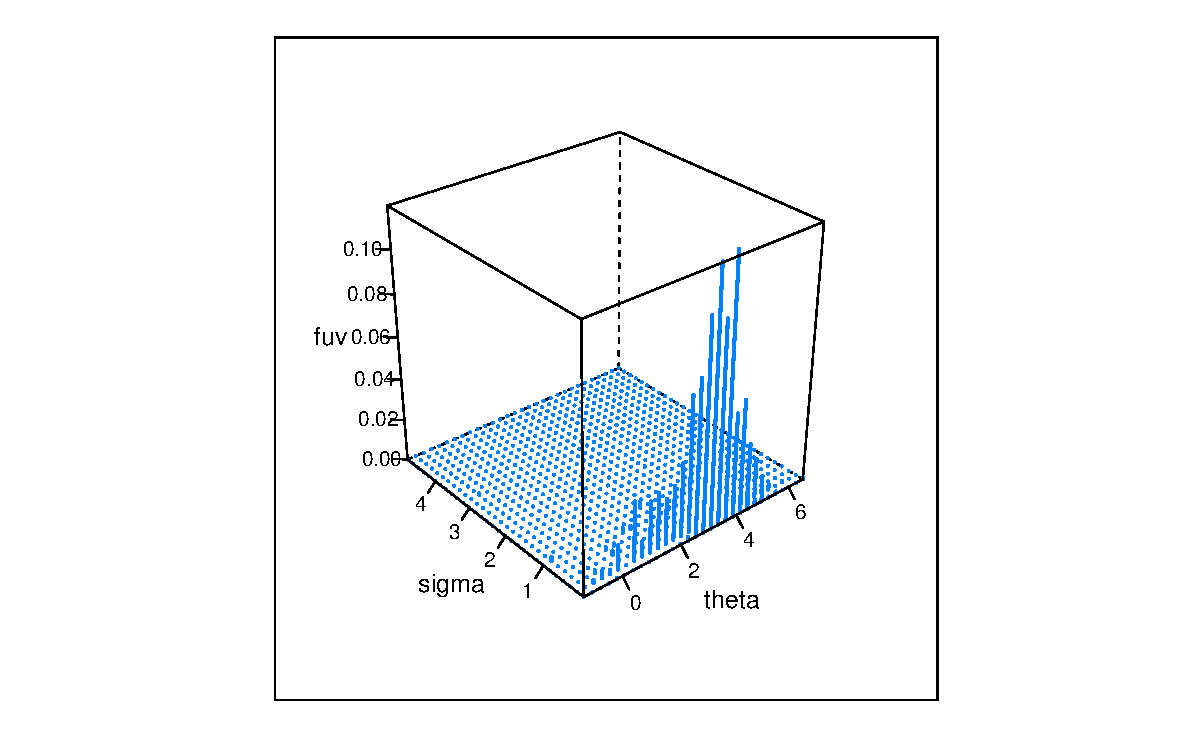
\includegraphics[width=\textwidth]{../../Figures/2013-2022/GMM_fd/GLVmix.pdf}
    \end{minipage}\hfill
    \begin{minipage}{0.5\textwidth}
        \centering
        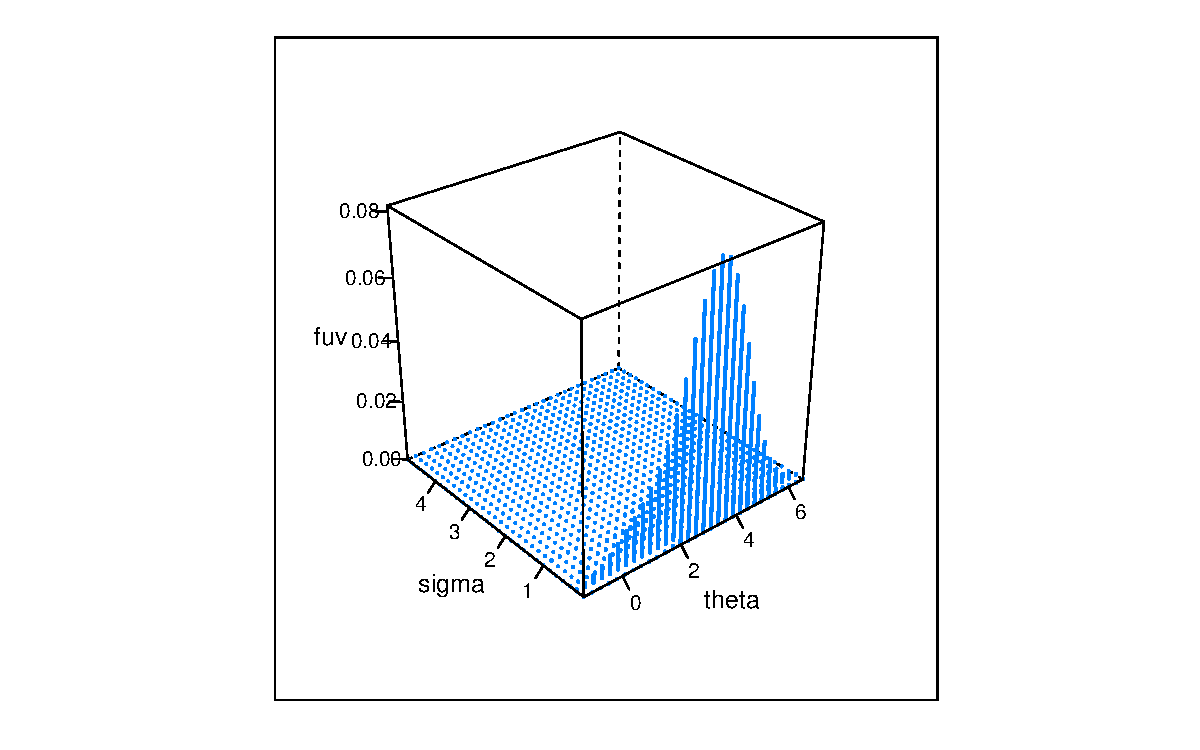
\includegraphics[width=\textwidth]{../../Figures/2013-2022/GMM_fd/GLVmix_s.pdf}
    \end{minipage}
    \label{fig:GLVmix}
\end{figure}

With an estimated prior, the tail probability function as well as the
constraints are well-defined. However, given the discrete nature of selection,
it resembles knapsack discrete optimization problem similar. I follow the
approach described in \cite{basu2018weighted} and thus consider only
sequentially selecting the units until one constraint is violated.

In Figure \ref{fig:tp_0.2_0.2_2d}, I present the results of selecting the top
20\% of hospitals with or without the FDR constraint set at 20\%. The selection
rule is the posterior tail probability, which is explained in the sections
above, that is, the solution to the problem defined in \ref{eq:decisionrule}.
The prior $G$ is taken to be the smoothed Kiefer-Wolfowitz estimate.

The left-hand side corresponds to the selection outcome without imposing the
FDR constraints, while the right-hand side controls the expected FDR at 20\%.
In the first case, there are around 10 times more private hospitals in the top
20\%, while the total number of hospitals is less than twice that of the
public.

The FDR seems to have impacted only the private hospitals, leaving 18 out of
the selection set. A more stringent FDR constraint would lead to a smaller set,
as shown in \ref{fig:tp_0.2_0.1_2d}.

\begin{figure}[h!]
    \centering
    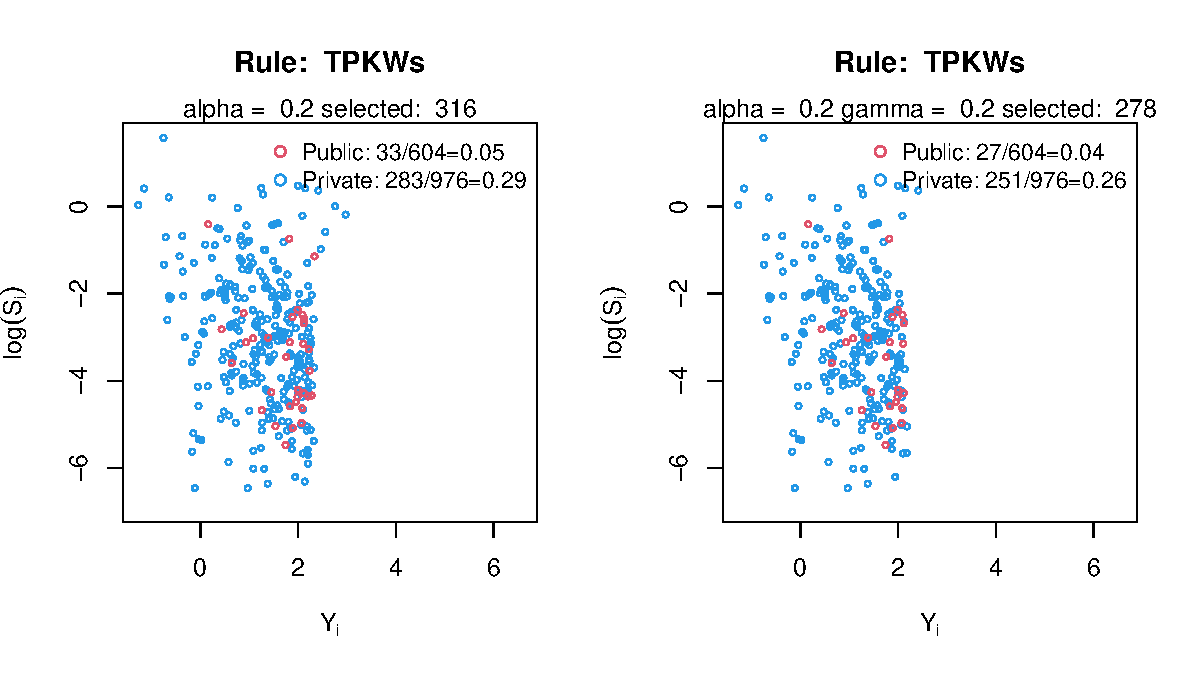
\includegraphics[width=0.8\textwidth]{../../Figures/2013-2022/GMM_fd/GLVmix/Left_0.2_0.2_TPKWs.pdf}
    \caption{Tail probability rule, capacity 20\%, FDR 20\%, unknown variance}
    \label{fig:tp_0.2_0.2_2d}
\end{figure}

\begin{figure}[h!]
    \centering
    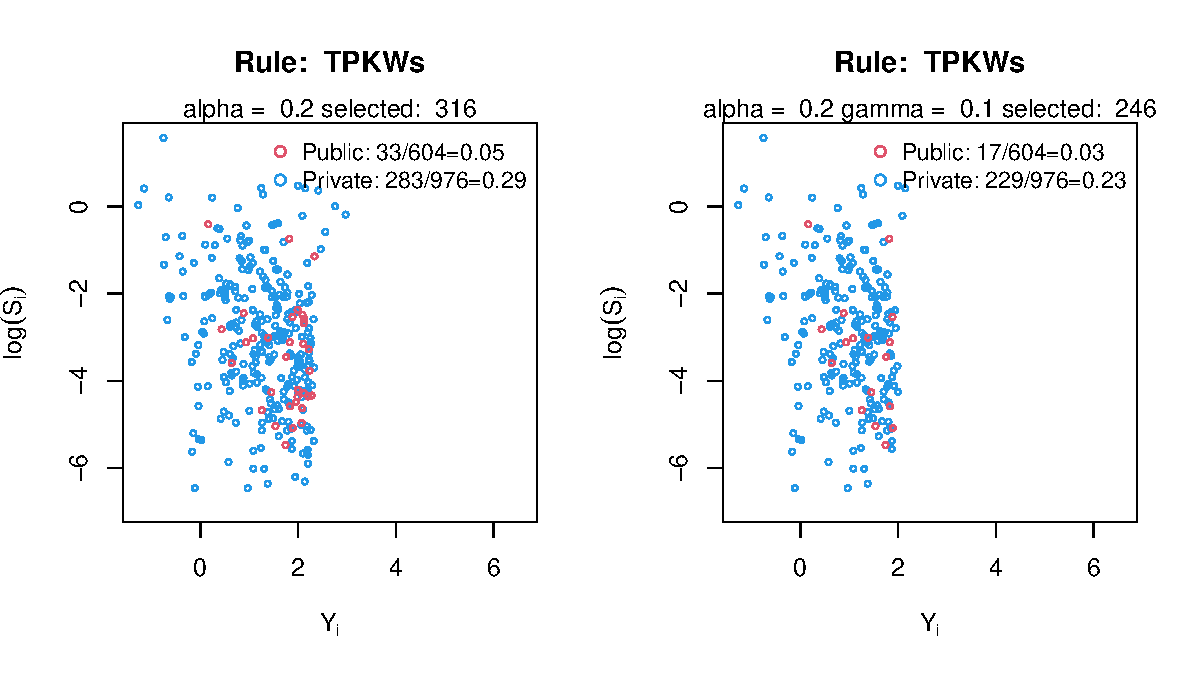
\includegraphics[width=0.8\textwidth]{../../Figures/2013-2022/GMM_fd/GLVmix/Left_0.2_0.1_TPKWs.pdf}
    \caption{Tail probability rule, capacity 20\%, FDR 10\%, unknown variance}
    \label{fig:tp_0.2_0.1_2d}
\end{figure}

For an overview of other selection rules using different ranking statistics,
such as the posterior mean, MLE face value, and James-Stein linear shrinkage,
see Appendix \ref{section:unknown}.

\
\paragraph{Known variance, and TP rules}

In \citet{gu2023invidious}, the authors apply the newly proposed selection
method to the selection of kidney dialysis centers, a topic previously studied
by \citet{lin2006loss, lin2009ranking}. However, their focus is on the quality
of service, specifically on the mortality rate. Furthermore, they assume that
the predictions of expected mortality are sufficiently accurate such that the
variance is known, independent of $\theta \sim G$.

Figure \ref{fig:GLmix} shows the estimated $\hat{G}(\theta)$ before and after
smoothing.

\begin{figure}[h!]
    \centering
    \begin{minipage}{0.5\textwidth}
        \centering
        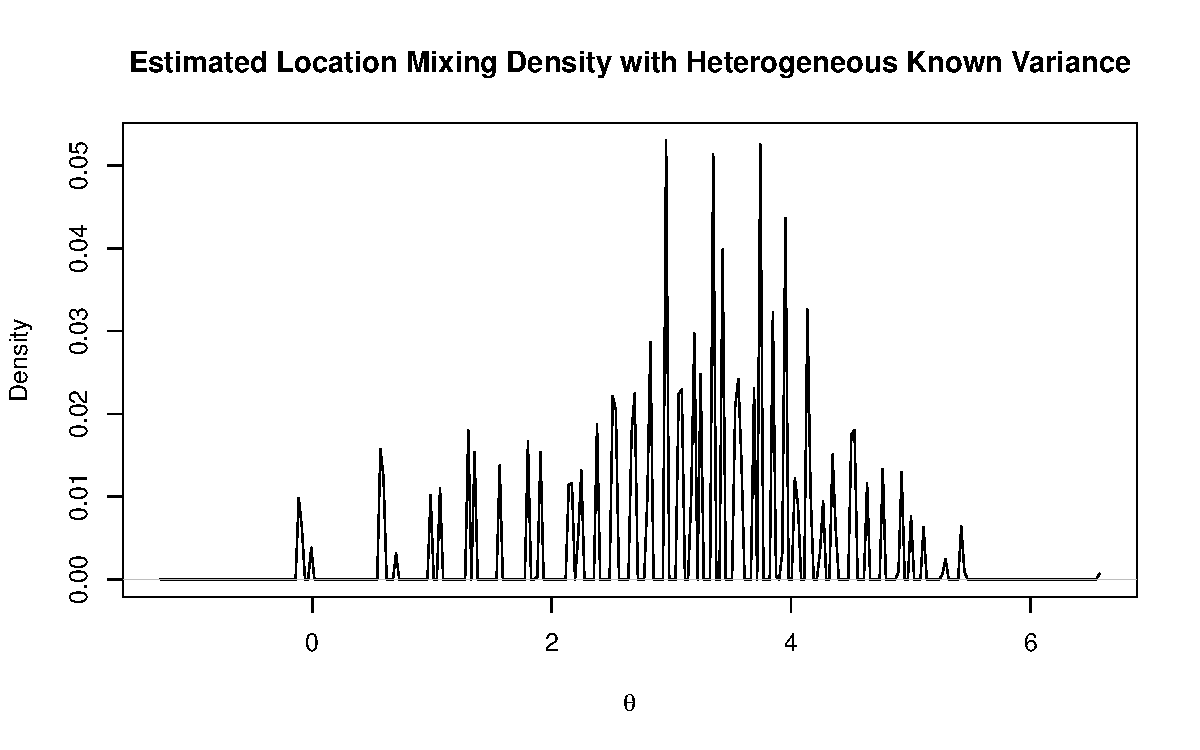
\includegraphics[width=\textwidth]{../../Figures/2013-2022/GMM_fd/GLmix.pdf}
    \end{minipage}\hfill
    \begin{minipage}{0.5\textwidth}
        \centering
        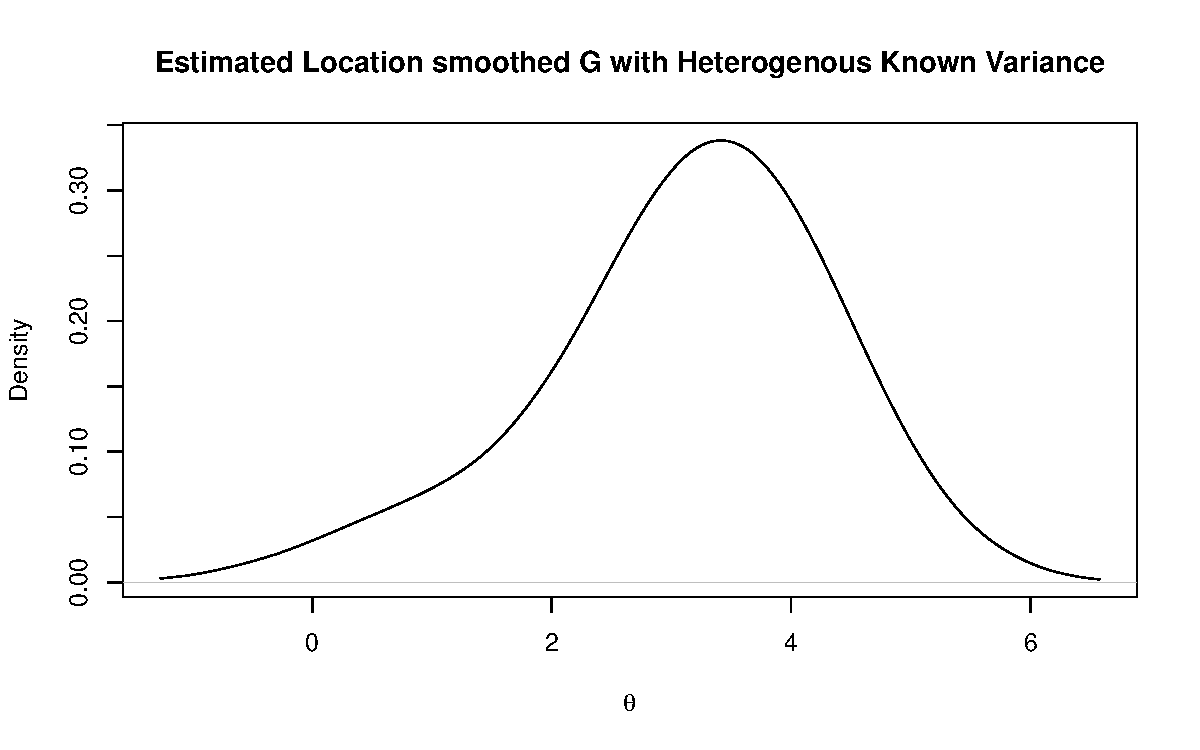
\includegraphics[width=\textwidth]{../../Figures/2013-2022/GMM_fd/GLmix_s.pdf}
    \end{minipage}
\end{figure}

Though not desirable in the present setting, it would be interesting to see
what the results would be if I take the $S_i$ as the $\sigma_i^2$. For the
moment, whether this assumption would lead to a more stringent selection
outcome is unclear. Figure \ref{fig:tp_0.2_0.2_1d} presents the outcome under
the posterior tail probability rule with a smoothed estimated prior. It seems
that with only the capacity constraint, the outcome does not differ much.
However, when an FDR constraint is combined, the known variance assumption
becomes too lenient to incorporate the newly imposed constraint. At the level
$\alpha=0.2$ and $\gamma=0.2$, the FDR constraint is not binding. However, a
more stringent FDR constraint at $\gamma=10\%$ does bind, as shown in Figure
\ref{fig:tp_0.2_0.1_1d}.

\begin{figure}[h!]
    \centering
    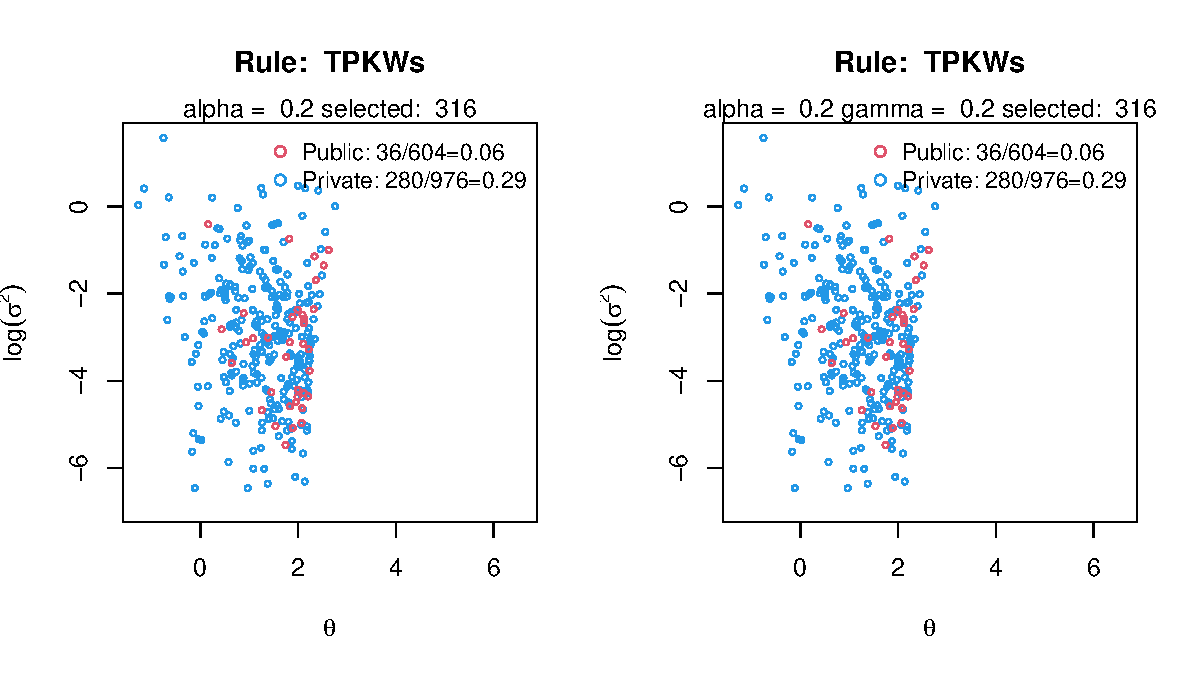
\includegraphics[width=0.8\textwidth]{../../Figures/2013-2022/GMM_fd/GLmix/Left_0.2_0.2_TPKWs.pdf}
    \caption{Tail probability rule, capacity 20\%, FDR 20\%, known variance}
    \label{fig:tp_0.2_0.2_1d}
\end{figure}

\begin{figure}[h!]
    \centering
    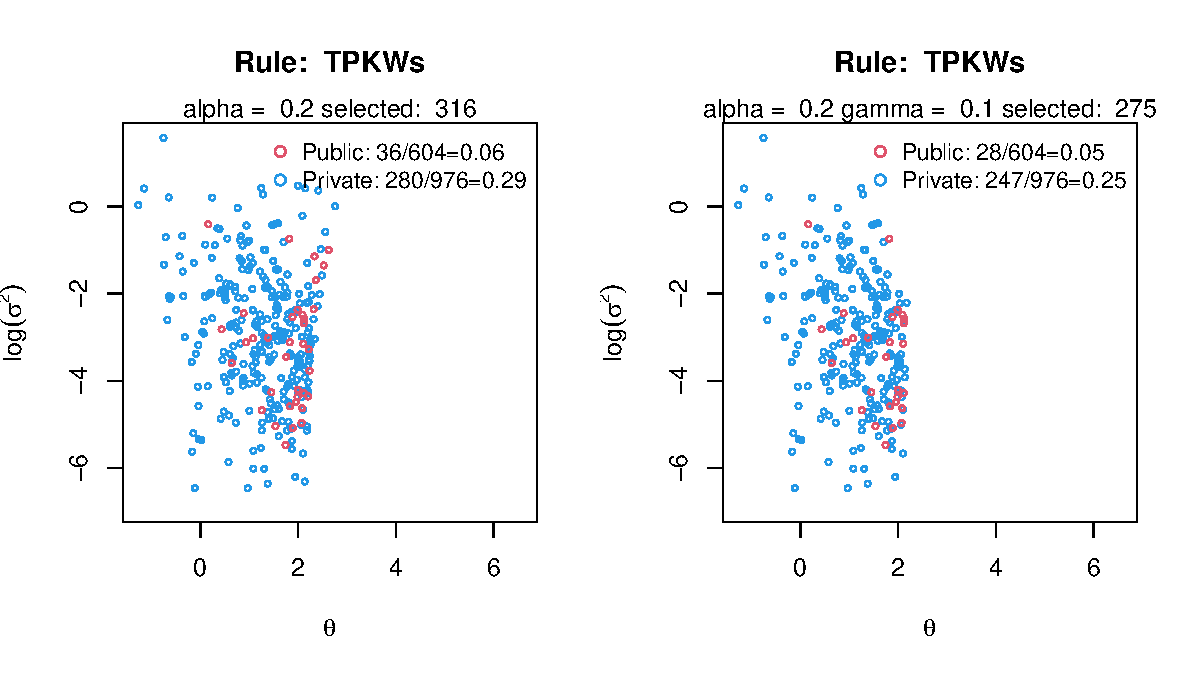
\includegraphics[width=0.8\textwidth]{../../Figures/2013-2022/GMM_fd/GLmix/Left_0.2_0.1_TPKWs.pdf}
    \caption{Tail probability rule, capacity 20\%, FDR 10\%, known variance}
    \label{fig:tp_0.2_0.1_1d}
\end{figure}

Appendix \ref{section:known} presents the results of other selection rules. In
this case, a contour line can be drawn to highlight the differences between
ranking statistics.

\section{Conclusion}
Exploiting the rich dataset covering all hospitals in France, I have attempted
to estimate the fixed effect of individual hospitals, which has the
interpretation of an \textit{inefficiency index}. Based on an initial estimate,
my goal is to select the top-performing hospitals and classify them by legal
status, thereby having a more granular view of the efficiency comparison
between public and private hospitals. I deliberately omit the teaching
hospitals (approximately 200) from the dataset because they inherently differ
in terms of objectives. To tackle the endogeneity issue, I used the lagged
difference of the regressors as instruments for the current level, a simplified
version of the system GMM method. The selection problem of interest falls
naturally under the compound decision framework. The Empirical Bayes ideology,
along with developments in nonparametric maximum likelihood estimation, has
made the implementation more efficient. In addition to the artificial capacity
constraint where only the top $\alpha\%$ of units are of interest, it is an
interesting and useful practice to incorporate another constraint called the
False Discovery Rate (FDR) constraint such that the expected number of false
positives is controlled at a certain level. From the application to French
hospitals, it is clear that the FDR constraint shrinks the selection set by
some amount. It is also intuitive that the larger the capacity (the larger the
$\alpha$), the less binding the FDR constraint is. The idea is that when the
decision-maker can select more units, the probability of making mistakes
decreases. Another observation comes from the assumption we make in the NPMLE
of $G$. In \citet{gu2023invidious}, the authors have pointed out that while the
known variance assumption in $Y_i|\theta_i,\sigma_i$ may be plausible in some
applications, it is more common to be faced with only an estimate of the
variance. The two assumptions give rise to a different level of
\textit{stringency} in response to the constraints, especially when the
decision-maker wants to control for the expected false discovery rate. Assuming
an unknown variance treats the observation as noisier, thus increasing the
probability of making mistakes. The same level of FDR constraint of 20\% only
binds in the unknown variance scenario. With respect to the private-public
comparison, among the top 20\% performers, there are around ten times more
private than public hospitals, while the ratio of total number is 5 to 3. A
preliminary conclusion is that in terms of labor employment efficiency, there
are more efficient private hospitals among the top performers. It may be of
interest to healthcare authorities to perform such selections and take
corresponding actions with respect to the selection outcome. From my point of
view, a related report based on the ranking and selection results will create
an incentive for healthcare providers to ensure the completeness of data input.
However, one cautionary note is the interpretation of the fixed effect
estimate. Since the fixed effect captures all time-invariant components of the
unit, whether it is only the unobserved heterogeneity of individual hospitals
or an actual measure of inefficiency is questionable. This issue is discussed
in \citet{greene2005fixed}. Lastly, despite the fact that it is human nature to
construct rankings and make selections, every step of the procedure requires
attention to specification, identification, and justifiable assumptions.
Incorporating constraints such as FDR in defining the problem may be helpful,
but the decision is still subject to great uncertainty and should be made with
caution and justification.

\pagebreak
\newpage
\bibliography{ref.bib}

\appendix
\section{Appendix}
\subsection{Data}

The panel is first filtered by the following criteria
\begin{enumerate}
    \item the number of nurses is positive,
    \item at least one of STAC inpatient, STAC outpatient, Sessions is positive,
    \item the number of observations is larger than 6
\end{enumerate}
Second, I add one to every variable to avoid null value when taking log.

\subsection{NPMLE $G$}
\citet{koenker2014convex} defined the primal problem as
\begin{equation*}
    \min_{f=dG}\set{-\sum_i \log g(y_i)\bigg |g(y_i) = T(f),\ K(f)=1,\ \forall i }
\end{equation*}
where $ T(f)=\int p(y_i |\theta)fd\theta $ and  $K(f)= \int f d\theta$.\\
By discretizing the support,
\begin{equation*}
    \min_{f=dG}\left\{-\sum_i \log g(y_i)\bigg |g=Af,\ {1^T}f=1\right\}
\end{equation*}
where $A_{ij}= p(y_i|\theta_j) $ and $ f = (f(\theta_1),f(\theta_2),\ldots,f(\theta_m))$.\\
It is straightforward to derive the dual problem
\begin{equation*}
    \max_{\lambda,\mu} \left\{ \sum_i \log \lambda_1(i) \bigg| A^T\lambda_1 < \lambda_2 1,\ (\lambda_1>0) \right\}
\end{equation*}

\subsection{Assumption on $\hat{\theta}_i|\theta_i,\sigma_i$}
If our specification and assumptions on exogeneity are correct, the consistency
of $\hat{\beta}$ is guaranteed by $N$'s asymptotic. However, our estimate of
the fixed effect is
\begin{align*}
    \hat{\theta}_i & =\frac{1}{T}\sum(\theta_i+\varepsilon_{it}+x_{it}(\beta-\hat{\beta}))              \\
                   & \overset{N\to \infty}{\longrightarrow} \theta_i+\frac{1}{T}\sum_t \varepsilon_{it} \\
\end{align*}
When $T$ is relatively small (or even fixed), I am not in a good position to use central limit theorem to claim that $\hat{\theta}_i \overset{d}{\to} \caln(\theta_i,\frac{\sigma_i^2}{T})$. A bold assumption that $\varepsilon_{it} \sim \caln(0,\sigma_i^2)$ will save me from the $T$ issue, which I will impose for the rest of the section (and abstract from whether that  for each $i$ is a testable/reasonable/feasible assumption).

\subsection{Comparison of selection rules}

\newpage
\subsubsection{Unknown variance}
\label{section:unknown}

\begin{figure}[h!]
    \centering
    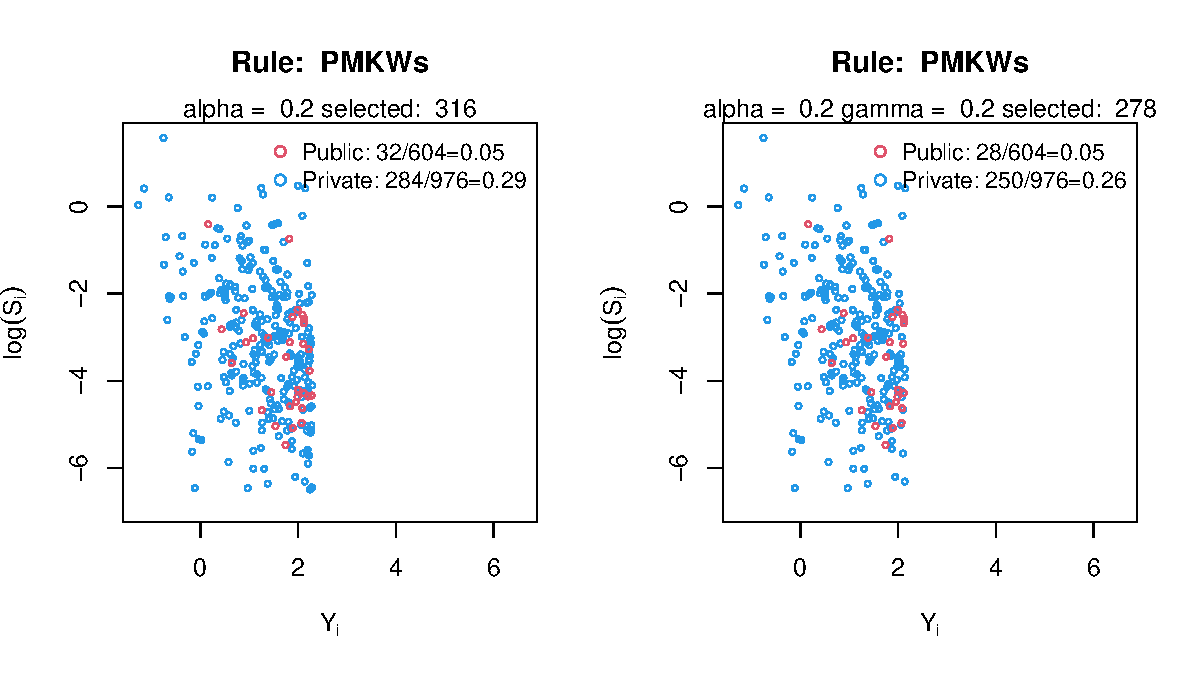
\includegraphics[width=0.8\textwidth]{../../Figures/2013-2022/GMM_fd/GLVmix/Left_0.2_0.2_PMKWs.pdf}
    \caption{Posterior mean, capacity 20\%, FDR 20\%, unknown variance}
\end{figure}

\begin{figure}[h!]
    \centering
    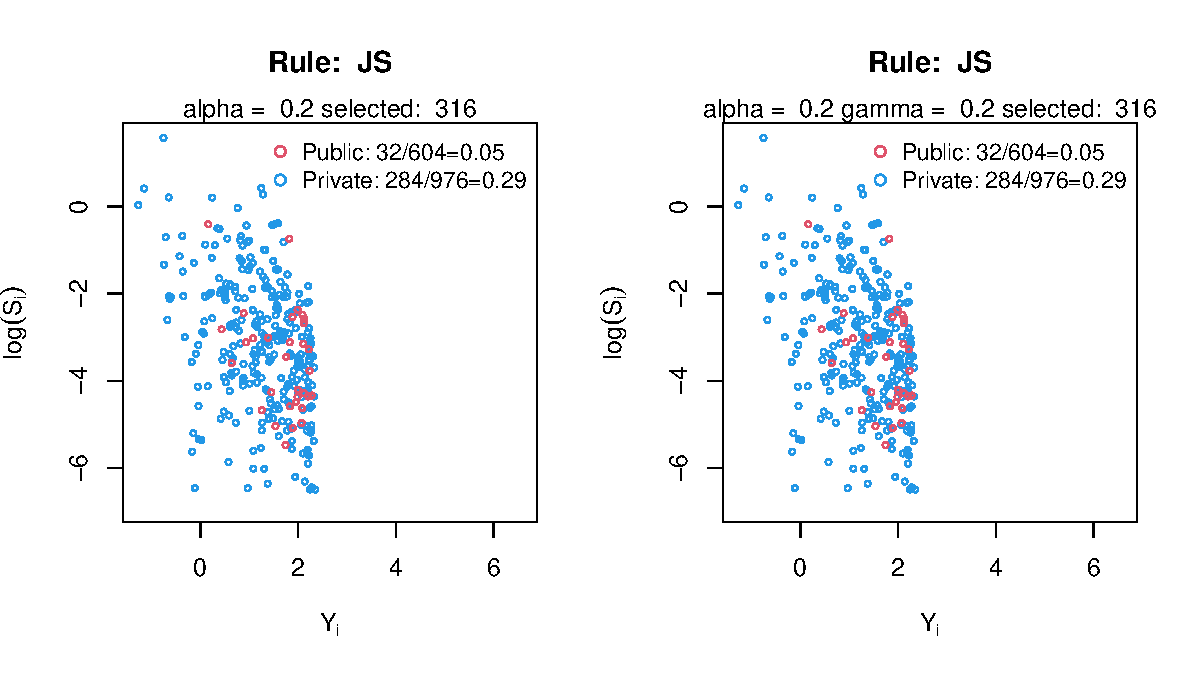
\includegraphics[width=0.8\textwidth]{../../Figures/2013-2022/GMM_fd/GLVmix/Left_0.2_0.2_JS.pdf}
    \caption{James-Stein Linear Shrinkage, capacity 20\%, FDR 20\%, unknown variance}
\end{figure}

\begin{figure}[h!]
    \centering
    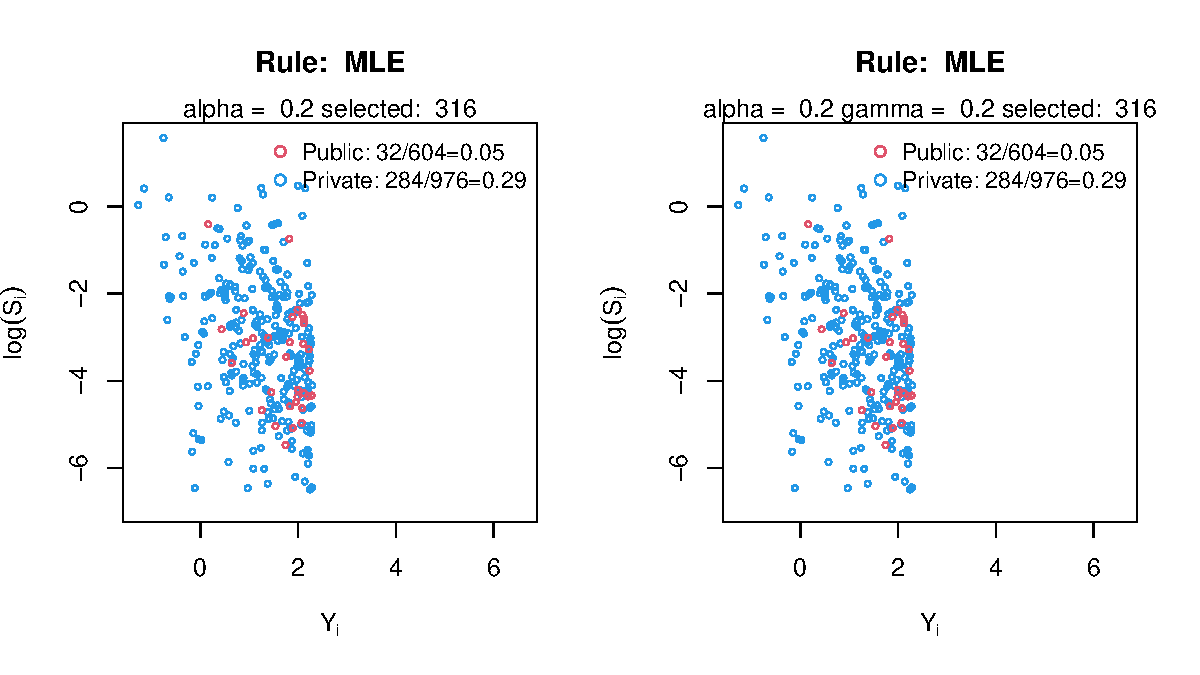
\includegraphics[width=0.8\textwidth]{../../Figures/2013-2022/GMM_fd/GLVmix/Left_0.2_0.2_MLE.pdf}
    \caption{MLE, capacity 20\%, FDR 20\%, known variance}
\end{figure}

\newpage
\subsubsection{Known variance}
\label{section:known}
\begin{figure}[h!]
    \centering
    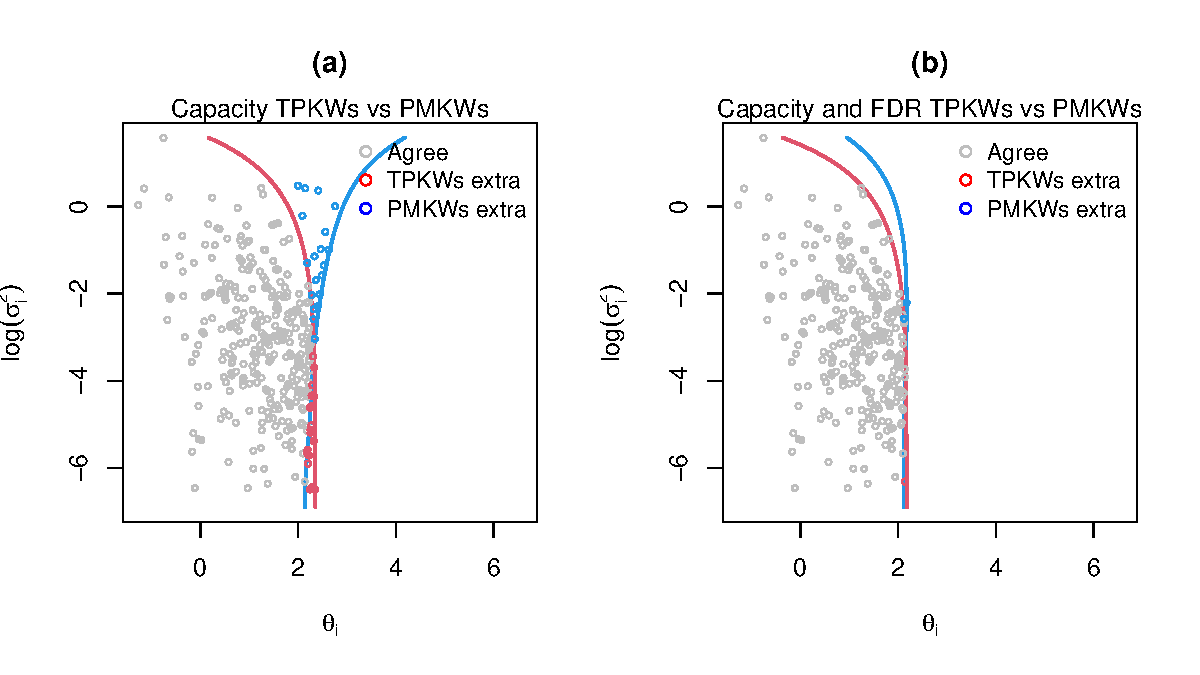
\includegraphics[width=0.8\textwidth]{../../Figures/2013-2022/GMM_fd/GLmix/Contour_Left_0.2_0.1_TPKWs_PMKWs.pdf}
    \caption{TP VS PM,  capacity 20\%, FDR 10\%, known variance}
\end{figure}

\begin{figure}[h!]
    \centering
    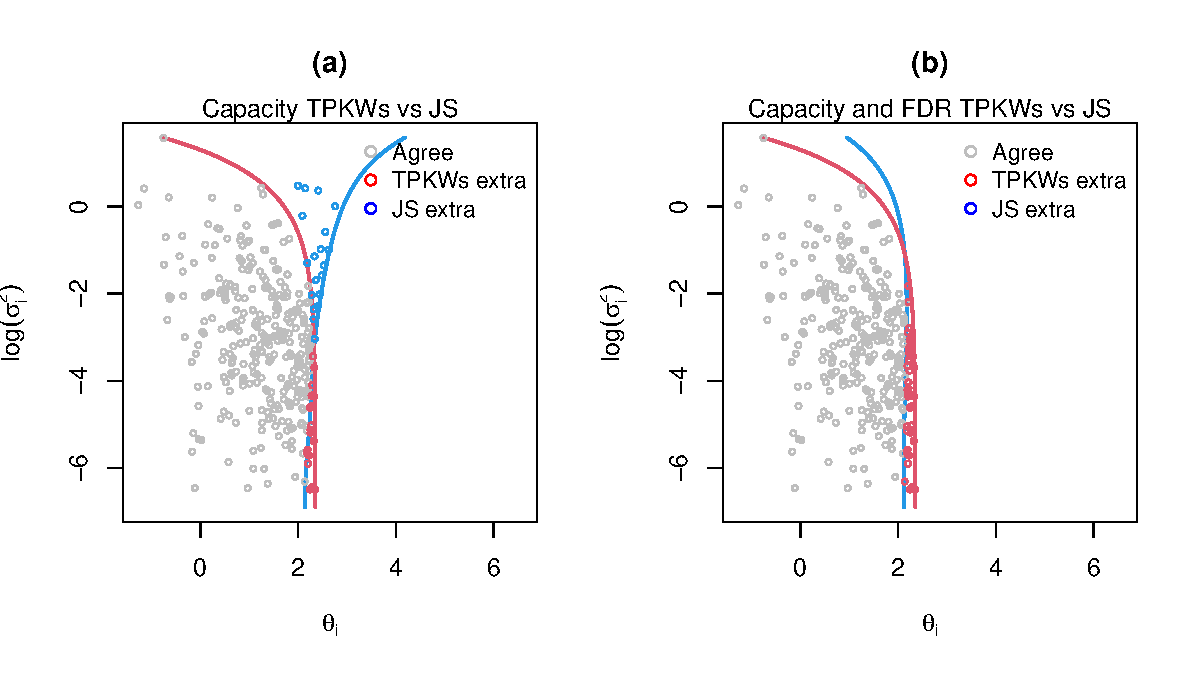
\includegraphics[width=0.8\textwidth]{../../Figures/2013-2022/GMM_fd/GLmix/Contour_Left_0.2_0.1_TPKWs_JS.pdf}
    \caption{TP VS JS, capacity 20\%, FDR 10\%, known variance}
\end{figure}

\begin{figure}[h!]
    \centering
    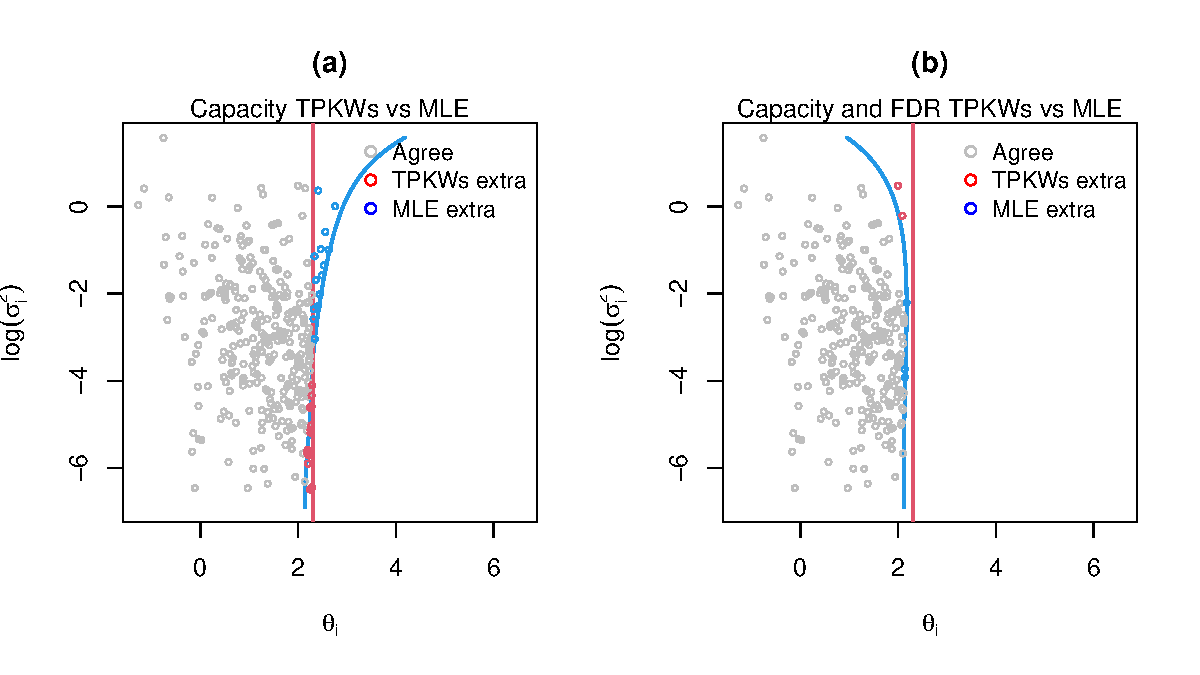
\includegraphics[width=0.8\textwidth]{../../Figures/2013-2022/GMM_fd/GLmix/Contour_Left_0.2_0.1_TPKWs_MLE.pdf}
    \caption{TP VS MLE, capacity 20\%, FDR 10\%, unknown variance}
\end{figure}

\end{document}